\documentclass[letterpaper,11pt]{article}

\usepackage{listings}
\usepackage{color}

\definecolor{dkgreen}{rgb}{0,0.6,0}
\definecolor{gray}{rgb}{0.5,0.5,0.5}
\definecolor{mauve}{rgb}{0.58,0,0.82}

\lstset{frame=tb,
  language=Python,
  aboveskip=3mm,
  belowskip=3mm,
  showstringspaces=false,
  columns=flexible,
  basicstyle={\small\ttfamily},
  numbers=none,
  numberstyle=\tiny\color{gray},
  keywordstyle=\color{blue},
  commentstyle=\color{dkgreen},
  stringstyle=\color{mauve},
  breaklines=true,
  breakatwhitespace=true,
  tabsize=3
}

\usepackage{setspace}
\usepackage{graphicx}
\usepackage{indentfirst}
\usepackage{bm}    %for textbf
\usepackage{amsmath}
\usepackage{amsfonts}   %for mathbb
\allowdisplaybreaks[4]  %from {amsmath}
\newcommand{\independent}{\rotatebox[origin=c]{90}{$\models$}}  %from {graphicx}
\usepackage{geometry}
\geometry{letterpaper, scale=0.8}  %from {geometry}
\author{Yuan Yin A20447290}
\title{MATH 584 Homework 1}
\begin{document}\large
\maketitle
\begin{spacing}{1.2}  %from {setspace}
\section*{Problem 1}
\subsection*{(a)}
I download data from Yahoo Finance with tickers given and date starting from 2009-01-01 to 2019-12-31. I only use the ``Adj Close'' part and I also check the data and there is no tickers with missing values. There are totally 64 assets and with 2768 days of prices. Then I compute the daily return and named with ``Ret'' in Python code. Then compute and annualized the mean and convariance matrix and save in ``AnnualizedMean.csv'' and ``AnnualizedCovariance.csv'' separately.

\subsection*{(b)}
For this part I compute the minimal-variance portfolio using the code in template. I got the minimal-variance portfolio and save them in ``MinimalVarPort.csv''

\subsection*{(c)}
Now we compute the weights of optimal mean-variance portfolio with risk tolerance $1/\gamma = 1$. I save the portfolio in ``MeanVarPort.csv''. And I plot the weights here:

\begin{figure}[h] %h for head or t for top
\centering
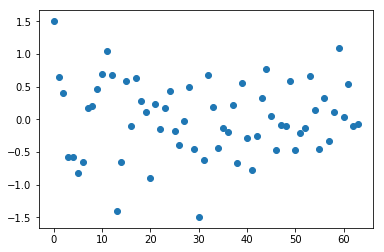
\includegraphics[scale=0.5]{1(c).png}
\caption{mean-var portfolio}
\label{fig:label}
\end{figure}

Notice that the portfolio mean is $2.142036414973624$ and portfolio variance is $1.0257049346650433$

\subsection*{(d)}
For this problem, I compute the weights of the optimal mean-variance portfolio in the robust setting. And I save the weights in ``MeanVarPortwRobust.csv'' file. And the plot of weight is as follows:

\begin{figure}[h] %h for head or t for top
\centering
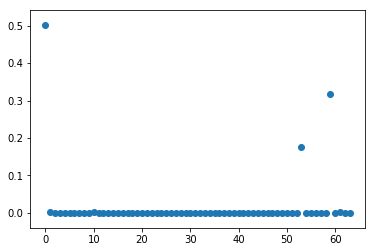
\includegraphics[scale=0.5]{1(d).png}
\caption{mean-var w. robust portfolio}
\label{fig:label}
\end{figure}

The variance of the portfolio is $0.041372046946460475$. And the best case mean is $0.5721439844938762$. The worst case mean is $0.05441305132035014$


Finding that for this problem our portfolio has lower mean with also lower variance than in problem 1(c), which makes sence since the robust method is to firstly find mean to minimize our objective function (making the worst case not so bad), thus the mean should be smaller than that in (c), and also since it's a robust method, the variance for the portfolio should be less than what in (c).

For the two graphs of weights, we can see that for robust method, our weights focus only on few assets, and the others are nearly zero weights. But for weights in (c), it's more dispersed. 

\subsection*{(e)}

Here is the plot for efficient frontier and pairs of individual basic assets:

\begin{figure}[h] %h for head or t for top
\centering
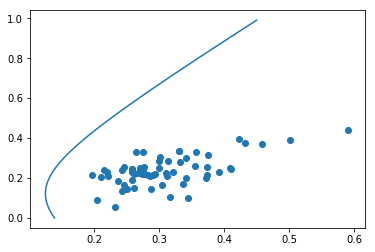
\includegraphics[scale=0.5]{1(e).png}
\caption{efficient frontier and basic assets}
\label{fig:label}
\end{figure}

Finding that all pairs are in the feasible set which is correct since for every fixed $\mu$, the minimal variance they can get is the efficient frontier, and all the others cases should lie to the right of the efficient frontier.

\subsection*{(f)}

Now adding riskless asset. I solve the linear system to firstly find market portfolio, and I save them in ``MarketPort.csv'' file. Then I compute the efficient frontier as for each give $\mu$, I compute the weight of riskless asset firstly and thus get the risky weight, which are proportionally to market portfolio we just compute and thus we get the whole portfolio. We can compute its mean and variance. The plot is as follows:

\begin{figure}[h] %h for head or t for top
\centering
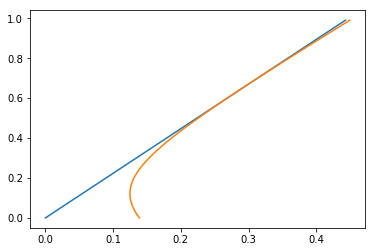
\includegraphics[scale=0.5]{1(f).png}
\caption{efficient frontier w. riskless asset}
\label{fig:label}
\end{figure}

The blue line is what we got the new efficient frontier with a riskless asset, and the orange one is what we got from (e). We can see that the blue line is the tangent line for the orange one, and it makes sence that we best portfolio we can combine with risky assets and riskless asset should be a tangent line for the efficient frontier of only risky assets.


\section*{Problem 2}
\subsection*{(a)}
I compute $\beta$ by the definition and save them in ``Beta.csv'' file.

\subsection*{(b)}
For this problem we use linear regression to get a CAPM model for our data. And I save the coefficients $\{(a_i,\beta_i)\}$ in ``LS\_pair.csv''.

By looking the results, we can find that $\{a_i\}$ are very nearly to zero and $\{\beta_i\}$ are almost the same to results in (a). It implies that our CAPM model is a reasonable in some way, which each asset is a proportion to the market.

\subsection*{(c)}
Now we consider one factor model with prior 5-day average return, I save coefficient for all assets in ``PriAve\_pair.csv'' file, with the first column representing $a_i$ and second column $c_i$. Then I print out all assets with p-value larger than significance level $0.05$, and I found that most of the assets have large p-value indicating that this factor may not be a good choice for one factor model.

\subsection*{(d)}
Now I use another factor which is volume-weighted prior 5-day average return. I save coefficients in ``VWPriAve\_pair.csv'' file with first column $a_i$ and second column $c_i$. Again, I print out assets number with p-values larger than significance level $0.05$ and there are around 40 assets not significant. I believe this factor is still not a good choice.

\subsection*{(e)}
Now we perform the regression with modification. We only focus on subsample of days which additional factor is above $\mu + \lambda\sigma$. And then we do the regression with diffierent choice of $\lambda$. And find the optimal one. I save the p-values for the optimal $\lambda$ in ``Pvalues.csv'' file with the first row for factor in (c) and second row for factor in (d).

Finally, I save the mean excess returns over the subsample and save them in ``ExcessRetMean.csv'' file, where the first row is for the factor in (c) and the second row is for factor in (d).

I also print out the values of mean excess returns of basic assets over the entire sample(not hedged). I found that the mean of hedged excess return of subsample is significantly smaller than entire sample. It is true since the coefficient for both factors are usually negative which means these factors has a negative effect on the excess return. Thus if we choose those subsamples with significantly larger factors, we would get smaller returns.

Then I compute the Sharpe Ratios for both subsamples with factors and entire samples. I found that the magnitude for subsamples over both factors are smaller than entire sample.

I also print out the size of all subsamples and we can see that the size is much smaller than the entire sample. This can largely decreases the time for regression in practice.

\end{spacing}
\end{document}